\subsection{Build RAVEN Input: \xmlNode{MultiRun}}
The \textbf{MultiRun} step allows the user to assemble the calculation flow of an analysis that requires multiple
``runs'' of the same model. This step is used, for example, when the input (space) of the model needs to be
perturbed by a particular sampling strategy. In the \xmlNode{MultiRun} input block, the user needs to specify the
objects that need to be used for the different allowable roles. This step accepts the following roles:

\begin{itemize}
  \item \textit{Input}
  \item \textit{Model}
  \item \textit{Output}
  \item \textit{Sampler}
  \item \textit{Optimizer}
  \item \textit{SolutionExport}
\end{itemize}

\textbf{MultiRun} is intended to handle calculations that involve multiple runs of a driven code (sampling strategies).
Firstly, the RAVEN input file associates the variables to a set of PDFs and to a sampling strategy. The ``multi-run''
step is used to perform several runs in a block of a model (e.g. in a MC sampling).

\begin{figure}[ht]
  \centering
  \includegraphics[width=0.8\textwidth]  {pics/MultiRunCalculationFlow.png}
  \caption{Calculation flow for a multi-run sampling}
  \label{fig:multiRun}
\end{figure}

As shown in Figure~\ref{fig:multiRun}, at the beginning of each sub sequential run, the sampler provides the new values of the variables to be perturbed.
The code API places those values in the input file. At this point, the code API generates the run command and asks
to be queued by the job handler. The job handler manages the parallel execution of as many runs as possible within
a user prescribed range and communicates with the step controller when a new set of output files are ready to be
processed. The code API receives the new input files and collects the data in the RAVEN internal format. The sampler
is queried to assess if the sequence of runs is ended, if not, the step controller asks for a new set of values
from the sampler and the sequence is restarted.
The job handler is currently capable to run different run instances of the code in parallel and can also handle
codes that are multi-threaded or using any form of parallel implementation.
RAVEN also has the capability to plot the simulation outcomes while the set of sampling is performed and to store
the data for later recovery.

In this section, we will show the user how to set up the \textit{Sampler}, and employ \textbf{MultiRun} to execute
all perturbed models. The use of \textit{Optimizer} and \textit{SolutionExport} will be introduced in another section.
The \textbf{Samplers}  entity is the container of all the algorithms designed to perform the perturbation of the
input space. The Samplers can be categorized into three main classes:

\begin{itemize}
  \item  \textit{Forward}. Sampling strategies that do not leverage the information coming from already evaluated
    realizations in the input space. For example, Monte-Carlo, Stratified (LHS), Grid, Response Surface, Factorial Design,
    Sparse Grid, etc.
  \item  \textit{Adaptive}. Sampling strategies that take advantages of the information coming from already evaluated
    realizations of the input space, adapting the sampling strategies to key figures of merits. For example, Limit Surface
    search, Adaptive sparse grid, etc.
  \item \textit{Dynamic Event Tree}. Sampling strategies that perform the exploration of the input space based on the
    dynamic evolution of the system, employing branching techniques. For example, Dynamic Event Tree, Hybrid
    Dynamic Event Tree, etc.
\end{itemize}

The sampler is probably the most important entity in the RAVEN framework. It provides many different sampling
strategies that can be used in almost all RAVEN related applications. In this section, we will only illustrate
the simplest forward sampler, i.e. \textit{Monte-Carlo}, to familarize the user with the use of sampler. Monte-Carlo method
is one of the most-used methodologies in several mathematic disciplines. The theory of this method can be found in
the RAVEN theory manual. In addition, we will continue to use the \textbf{AnalyticBateman} to illustrate the setup
of \textbf{MultiRun} and \textbf{Samplers}. In order to accomplish these tasks, the following precedures are needed:

\begin{enumerate}
  \item Set up the running environment: \xmlNode{RunInfo}
  \item Provid the required files: \xmlNode{Files}
  \item Link between RAVEN and dirven code: \xmlNode{Models}
  \item Define probability distribution functions for inputs: \xmlNode{Distributions}
  \item Set up a simple Monte-Carlo sampling for perturbing the input space: \xmlNode{Samplers}
  \item Store the input and output data: \xmlNode{DataObjects}
  \item Print and plot input and output data: \xmlNode{OutStreams}
  \item Control multiple executions: \xmlNode{Steps}
\end{enumerate}

In section~\ref{sub:singleRun}, we have already discussed the use of \xmlNode{RunInfo}, \xmlNode{Files}, \xmlNode{Models},
\xmlNode{DataObjects}, \xmlNode{OutStreams}. For practice, the user can try to build these RAVEN entities by themselves,
and refer to the complete input file located at
\textit{raven/tests/framework/user\_guide/ ForwardSamplingStrategies/forwardSamplingMontecarlo.xml}.
In this section, we'd like to show the users how to set up \xmlNode{Distributions}, \xmlNode{Samplers} and \textbf{MultiRun}
of \xmlNode{Steps}. RAVEN employs \xmlNode{Distributions} to define many different probability distribution
functions (PDFs) that can be used to characterize the input parameters. One can consider the \xmlNode{Distributions}
entity to be a container of all the stochastic representation of random variables. Currently, RAVEN supports:
\begin{itemize}
  \item \textit{1-Dimensional} continuous and discrete distributions, such as Normal, Weibull, Binomial, etc.
  \item \textit{N-Dimensional} distributions, such as Multivariate Normal, user-inputted N-Dimensional distributions.
\end{itemize}
For the \textbf{AnalyticBateman} example, two 1-D uniform distributions are defined:
\begin{itemize}
  \item $sigma \sim \mathbb{U}(1,10)$, used to model the uncertainties associated with the \textit{sigma} Model variables;
  \item $decayConstant \sim \mathbb{U}(0.5e-8,1e-8)$,  used to model the uncertainties associated with the Model variable
    \textit{decay constants}.  Note that the same distribution can be re-used for multiple input variables, while
    still keeping those variables independent.
\end{itemize}
The following is the definition of \xmlNode{Distributions} block that is used for the \textbf{AnalyticBateman} problem:
\xmlExample{framework/user_guide/ForwardSamplingStrategies/forwardSamplingMontecarlo.xml}{Distributions}
For uniform distributions, only \xmlNode{lowerBound} and \xmlNode{upperBound} are required.

As we already mentioned, we will employ Monte-Carlo sampling strategy to demonstrate \textbf{MultiRun}.
To employ the Monte-Carlo sampling strategy, a \xmlNode{MonteCarlo} node needs to be defined.
The user also needs to specify the variables that need to be sampled using \xmlNode{variable}. In addition,
the setting for this sampler need to be specified in the \xmlNode{samplerInit} block. The only required sub-node
\xmlNode{limit} is used to specify the number of Monte Carlo samples. The user can also use other optional sub-node
to characterize their samplers. For this example, the \xmlNode{Samplers} block is:
\xmlExample{framework/user_guide/ForwardSamplingStrategies/forwardSamplingMontecarlo.xml}{Samplers}
In this case, the Monte-Carlo method is employed on $eight$ model variables, each of which are listed by name and
are associated with a distribution. Note that all the \textit{decay-\*} and \textit{sigma-\*} variables are
associated with the distributions $decayConstant$ and $sigma$, respectively.

Once all the other entities are defined in the RAVEN input file, they must be combined in the \xmlNode{Steps} block,
which dictates the workflow of RAVEN.  For this case, two \xmlNode{Steps} are defined:
\begin{itemize}
  \item \xmlNode{MultiRun} ``sample'', used to run the multiple instances of the driven code and  collect the outputs
    in the two \textit{DataObjects}. As it can be seen, the \xmlNode{Sampler} is specified to communicate to the
    \textit{Step} that the driven code needs to be perturbed through the Monte-Carlo sampling.
  \item  \xmlNode{IOStep} named ``writeHistories'', used to 1) dump the ``histories'' and ``samples'' \textit{DataObjects}
    \textbf{Entity} to a CSV file and 2) plot the data in the EPS file.
\end{itemize}

Figures~\ref{fig:historiesMCPlotLine_A} and ~\ref{fig:samplesMCPlotLine_A} show the report generated by RAVEN of the
evolution of the variable $A$ and its final values, respectively.
%%%%%%%%%%%%%%%%%%%%%%%%%%%%%%%%%%%%%%%%%%%%%%%%%%%%%%%%%%
%figure histories
\begin{figure}[h!]
  \centering
  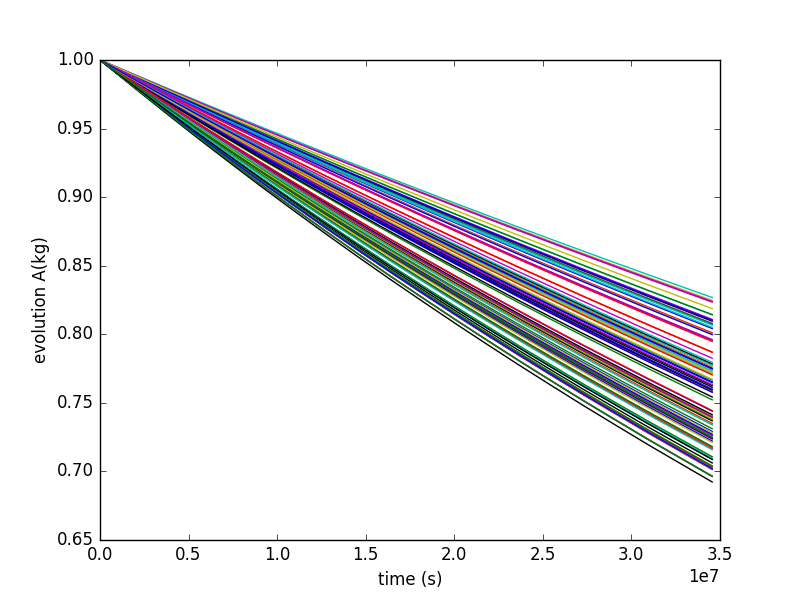
\includegraphics[scale=0.7]{../../tests/framework/user_guide/ravenTutorial/gold/MonteCarlo/1-history_A_line.png}
  \caption{Plot of the histories generated by the Monte Carlo sampling for variable $A$.}
  \label{fig:historiesMCPlotLine_A}
\end{figure}
%%%%%%%%%%%%%%%%%%%%%%%%%%%%%%%%%%%%%%%%%%%%%%%%%%%%%%%%%%
 
%%%%%%%%%%%%%%%%%%%%%%%%%%%%%%%%%%%%%%%%%%%%%%%%%%%%%%%%%%
%figure samples
\begin{figure}[h!]
  \centering
  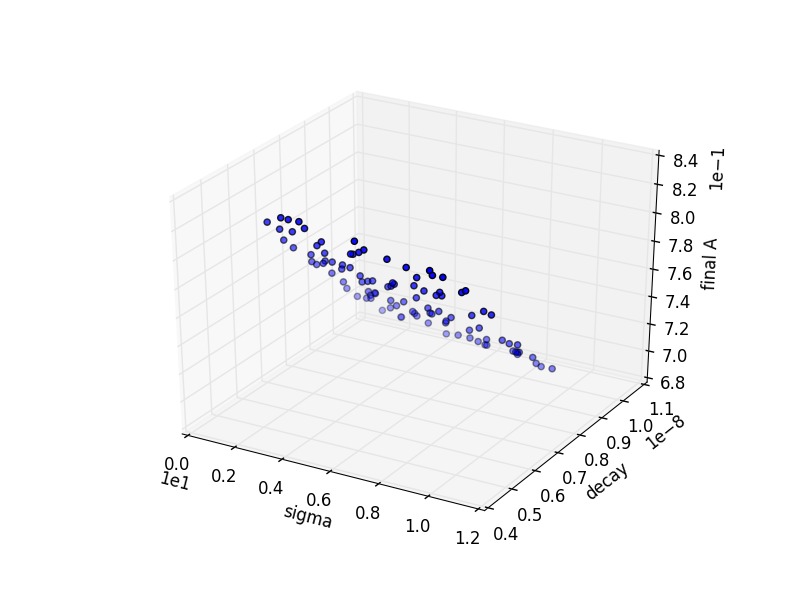
\includegraphics[scale=0.7]{../../tests/framework/user_guide/ravenTutorial/gold/MonteCarlo/1-samplesPlot_A_scatter.png}
  \caption{Plot of the samples generated by the MC sampling for variable $A$.}
  \label{fig:samplesMCPlotLine_A}
\end{figure}
%%%%%%%%%%%%%%%%%%%%%%%%%%%%%%%%%%%%%%%%%%%%%%%%%%%%%%%%%%
